\documentclass{standalone}
\usepackage{tikz}
\usepackage{ctex,siunitx}
\setCJKmainfont{Noto Serif CJK SC}
\usepackage{tkz-euclide}
\usepackage{amsmath}
\usetikzlibrary{patterns, calc,3d}
\usetikzlibrary {decorations.pathmorphing,decorations.pathreplacing,decorations.shapes}
\tikzset{label style/.append style={font=\small}}
\begin{document}
\small
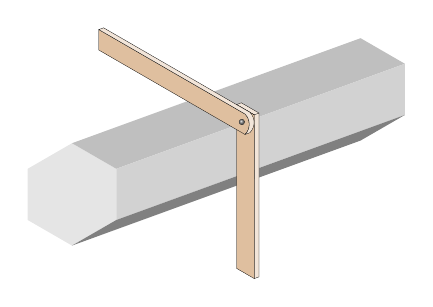
\begin{tikzpicture}[>=latex,scale=1.3,inner sep=2pt]
  \fill[lightgray!40](30:0.5)--(90:0.5)--(150:0.5)--(210:0.5)--(270:0.5)--(330:0.5)--cycle;
  \fill[lightgray](30:0.5)--++(20:3)--++(150:0.5)--++(20:-3)--cycle;
  \fill[lightgray!70](30:0.5)--++(20:3)--++(270:0.5)--++(20:-3)--cycle;
  \fill[gray](-30:0.5)--++(20:3)--++(-150:0.5)--++(20:-3)--cycle;
  \coordinate (A) at ([shift=(20:1.2cm)]30:0.5);
  \coordinate (B) at ([shift=(20:1.25cm)]30:0.5);
  \draw[ultra thin,fill=brown!20](B)--++(0,0.2)--++(20:0.05)--++(-30:0.2)--++(270:1.6)--++(20:-0.05)--++(90:1.5)--cycle;
  \draw[ultra thin,fill=brown!50]([shift=(90:0.2)]B)--++(270:1.6)--++(-30:0.2)--++(90:1.6)--cycle;
  \draw[ultra thin](B)--++(0,0.2)--++(-30:0.2)--++(20:0.05);
  \draw[ultra thin,fill=brown!50](A)--++(150:1.5)--++(90:0.2)coordinate(C)--++(-30:1.65)to[bend left=45]([shift=(-30:0.15)]A)--cycle;
  \coordinate (D) at ([shift=(-30:1.65)]C);
  \draw[ultra thin,fill=brown!20](D)--(C)--++(20:0.05)--++(-30:1.65)to[bend left=45]([shift=(-30:0.15)]B)--([shift=(-30:0.15)]A)to[bend right=45](D);
  \fill[ball color=gray]([shift=(30:0.06)]B)circle(0.8pt);
\end{tikzpicture}
\end{document}